\section{Maxim Gorkij}

\noindent
\textbf{28. března 1868 -- 18. června 1936}

\noindent
Vlastním jménem Alexej Maximovič Peškov, byl ruský spisovatel, dramatik, básník a revolucionář. Bývá považován za průkopníka socialistického realismu.

V roce 1879 osiřel a od té doby se musel živit víceméně samostatně, střídal různá zaměstnání a od 15 let (1883) se toulal po Rusku a vzdělával se. V této době se aktivně zapojil do revolučního hnutí. Po VŘSR odešel do emigrace, kde žil několik let, ale pak se na jednu ze Stalinových výzev vrátil. V Čechách (Mariánské Lázně 1923--1924) si léčil tuberkulózu.

Gorkij zcela jistě věděl o utrpení, které je Rusku způsobeno socialismem, ale přesto dál tento režim propagoval, nebylo to způsobeno strachem, mohl Rusko opustit, ale rozhodl se obětovat pravdu revoluci.

\podpis{http://www.wikipedia.cz}

\begin{center}
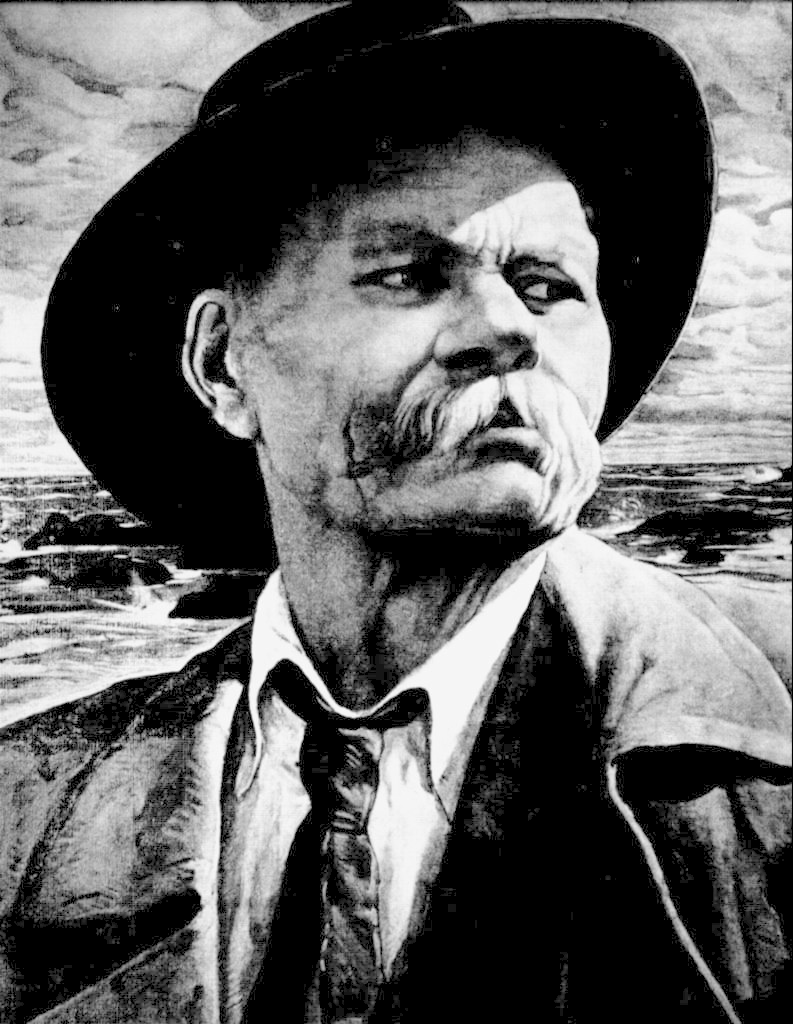
\includegraphics{plavrevue-34/obr/gorky.png}
\end{center}
